\chapter{Implementation}
\label{sec:implementation}

In order to conduct the experiments presented in this thesis,
a custom framework has been created in Python.
The source code is available at Github\footnote{\url{https://github.com/mathiasose/CA-NEAT/}}.
The system consists of a mix of library components and self-made components.

The CA subsystem was built from scratch.
It supports 1D and 2D grids with various border conditions (finite, toroidal, expanding), and should be easily extensible for other cases in the future.
For each problem there is a problem-specific fitness function which receives a genotype as input from the NEAT subsystem,
develops the transition function and iterates the CA  before evaluating the performance and returning a fitness value to the NEAT system.

The NEAT portion of the system is mostly based on the library \texttt{neat-python}\footnote{\url{https://github.com/CodeReclaimers/neat-python/}}.
Data structures for genomes and networks as well as various functions have been used without modifications.
The main evolutionary loop was re-implemented with modifications.
This was done for multiple reasons, including to take advantage of parallelism using \texttt{Celery}\footnote{\url{http://celeryproject.org/}} and to store the results in a database using \texttt{SQLAlchemy}\footnote{\url{http://sqlalchemy.org/}}.
Other software dependencies include \texttt{matplotlib}\footnote{\url{http://matplotlib.org/}} and \texttt{seaborn}\footnote{\url{http://seaborn.pydata.org/}} for visualization, and \texttt{dill}\footnote{\url{https://github.com/uqfoundation/dill}} for data and code serialization.

\section{CA-NEAT}
\begin{figure}
\centering
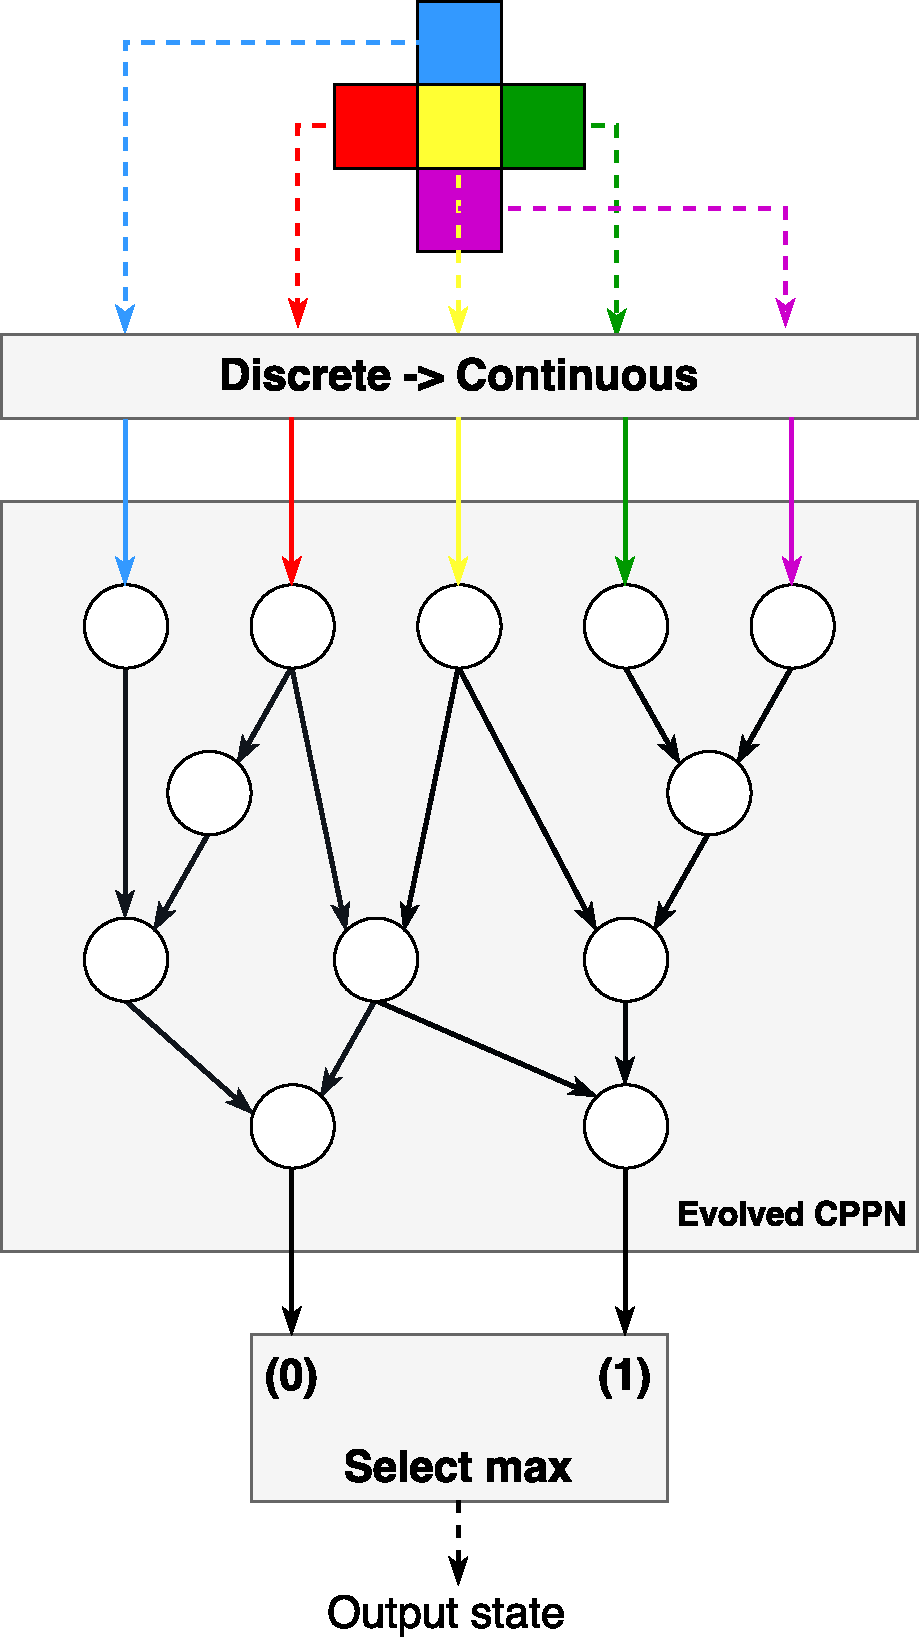
\includegraphics[width=.7\columnwidth]{fig/CA_NEAT}
\caption{
    Overview of how to use a CPPN as a CA transition rule.
    }
\label{fig:CA_NEAT}
\end{figure}

\begin{figure}
\centering
\begin{multicols}{3}
\begin{enumerate}
    \item Sigmoid
    \item Hyperbolic tangent
    \item Sinusoid
    \item Gaussian
    \item Rectified linear unit
    \item Identity
    \item Clamped
    \item Inverse
    \item Logarithmic
    \item Exponential
    \item Absolute value
    \item Hat
    \item Square
    \item Cube
\end{enumerate}
\end{multicols}
\caption{Possible activation functions}
\label{fig:activations}
\end{figure}

\begin{figure}
\centering
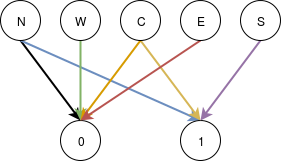
\includegraphics[width=.5\columnwidth]{fig/single_layer_cppn}
\caption
[Example first-generation CPPN with 7 out of 10 possible connections.]
{Example first-generation CPPN with 7 out of 10 possible connections. $N=5$ input nodes corresponds to the "Von Neumann" neighborhood shape, and $K=2$ output nodes correspond to a binary CA.}
\label{fig:single_layer_cppn}
\end{figure}

Since the \texttt{neat-python} library provides a NEAT implementation,
the majority of the development in this project consisted of creating the CA subsystem and the interfacing between CA code and NEAT code.

Figure \ref{fig:CA_NEAT} gives an illustrated overview of the mapping from neighborhood input to a new cell state.
The cell states are discrete values from a finite set,
but the activation functions used in the CPPN have expect inputs and outputs from the real numbers ($\mathbb{R}$).
Therefore there a mapping is performed before the CPPN input layer, assigning a continuous value to each possible cell state.
The mapping assigns each value in the finite state set to a value in the range $[-1.0, 1.0]$, evenly distanced.

The mapped values are then sent to the CPPN as input.
After the values have propagated through the network there are $K$ different outputs.
These are each paired with one of the cell states,
and the cell state corresponding to the CPPN output with the highest activation value is selected as the output and becomes the next state of the cell.

The activation functions used in the experiments in this thesis are listed in Figure \ref{fig:activations}.

The fitness evaluation function is specific to each problem.
In all experiments in this thesis, the fitness values returned are between 0 and 1, with 0 representing a complete failure and $1.0$ representing a perfectly accomplished task.

\subsection{Mapping CA-NEAT Encodings to Traditional Encodings}
\label{sec:behavior}
The mapping between the discrete and continuous number domains that happens before and after the CPPN is activated,
means that many CPPNs that are have different topologies, activation functions and weights,
will actually exhibit the exact same behavior as transition functions.
Enumerating all the possible inputs and recording the corresponding output of the transition functions creates a classical table/string representation of the transition functions.
We'll call this the \textit{behavior} of the transition function, and use this representation in analysis.

\subsection{Extending CPPN Input with Environmental Information}
\label{sec:input_extensions}
\begin{figure}
\centering
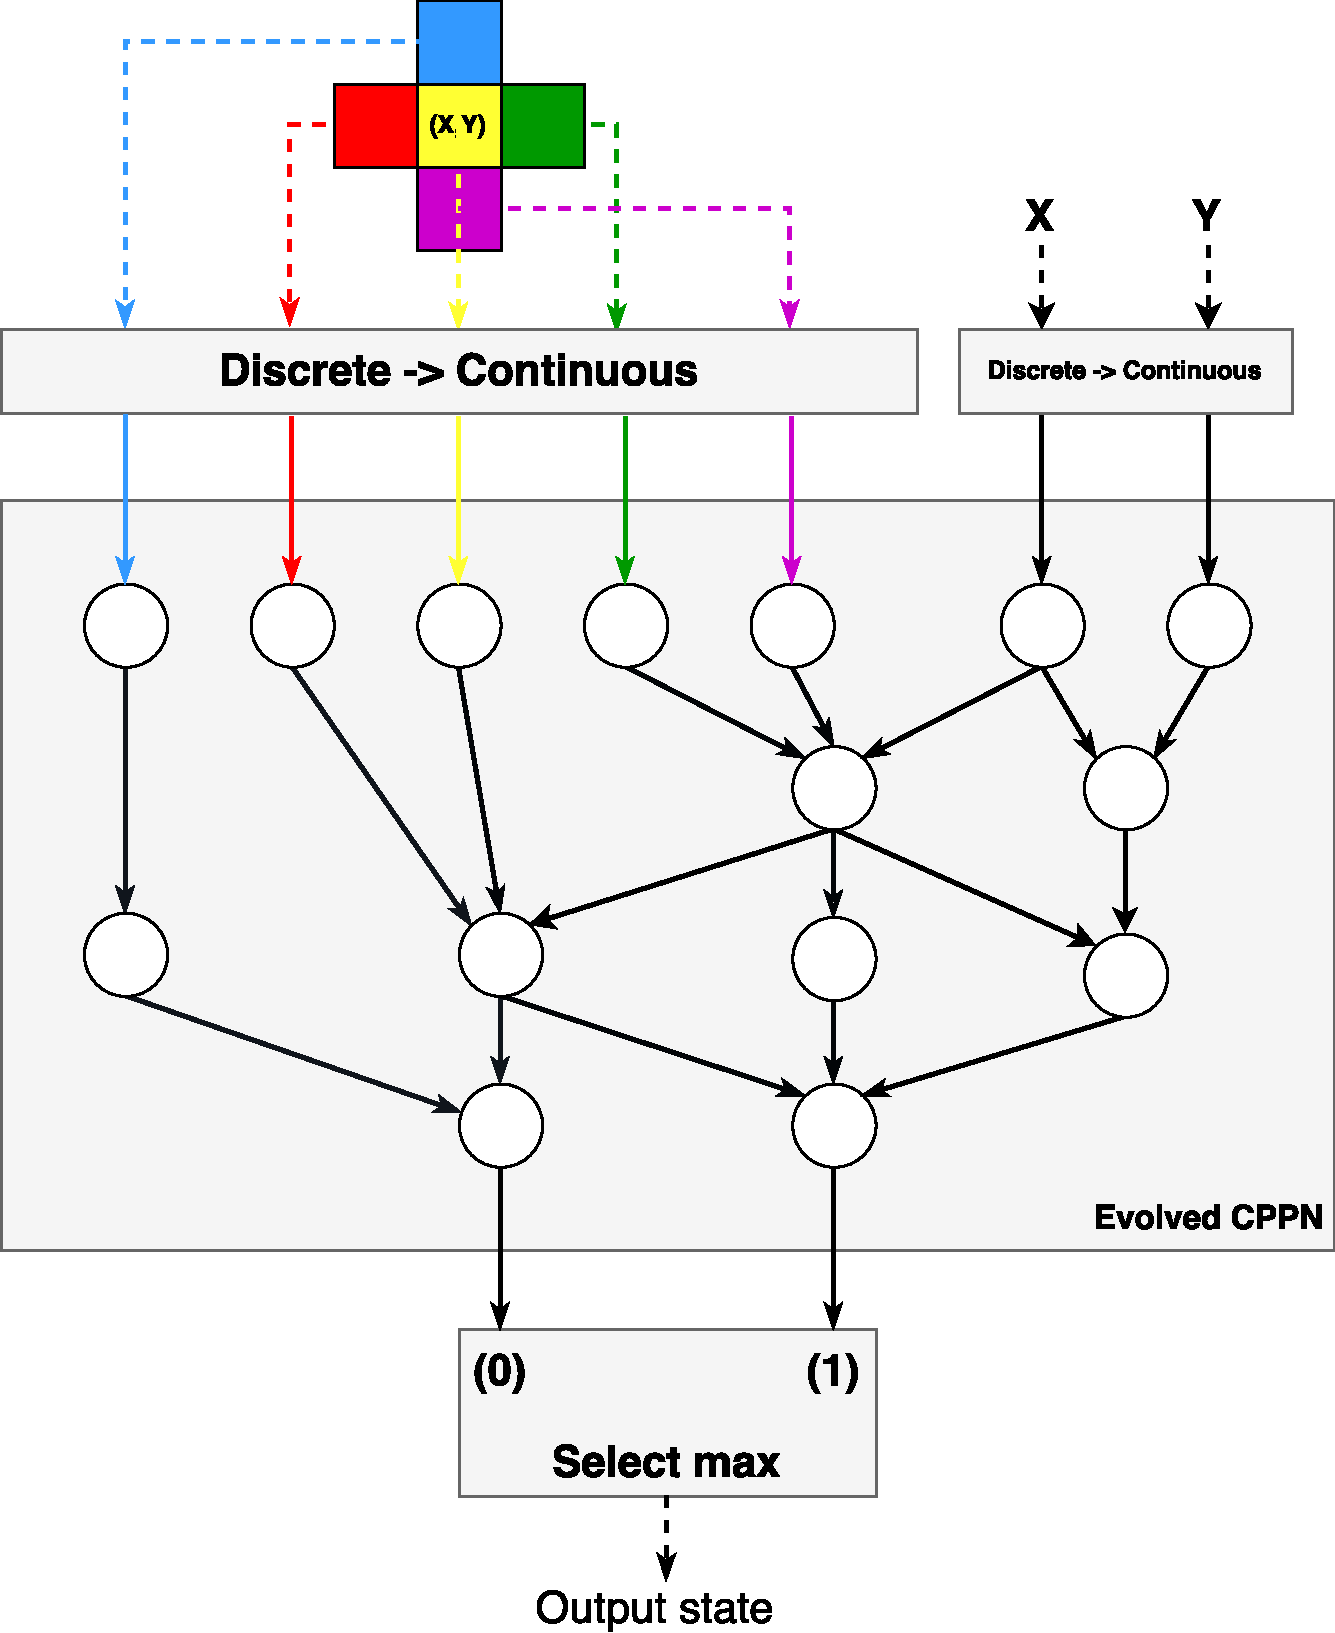
\includegraphics[width=.7\columnwidth]{fig/CA_NEAT_extension}
\caption{
    An example extension of CA-NEAT.
}
\label{fig:CA_NEAT_extension}
\end{figure}

Another aspect of CA-NEAT that can be explored, is the possibility of using inputs that are not neighboring states.
A table-based transition function is a complete mapping from all the possible inputs to a specific output.
A CPPN structure such as a CA-NEAT phenotype is less restricted in what kinds of inputs it can accept.

In biological cell systems, external factors can have large effects on the development.
For instance, a growing plant will choose which direction to expand in based on where it can find light or water in its environment.
In embryogenesis of animals,
spatial information is used to produce the correct layout of the body,
with brain cells forming in the head, skin cells on the surface of the body, and so on.
This is not all encoded in the genome of the organism, but arises from the interaction between the genome rules and the environment.

In a CA experiment, adding environmental information to the transition introduces a factor of indirect encoding,
since the same genotype can then produce different phenotypes in different environments.

Extending CA-NEAT to accept new kinds of inputs is very simple.
The NEAT part only needs to be told how many input nodes the networks should have.
Then the fitness evaluation function, which must be custom for each problem anyway,
must be programmed to extract the necessary values from the cellular model.

A concrete example is the extension used in the experiment in Section \ref{sec:morphXY}.
Figure \ref{fig:CA_NEAT_extension} illustrates this.
In addition to the neighborhood information, the coordinate values of the cell in question is also input to the network, which therefore has two additional input nodes.
The coordinate values are also mapped to the $[-1.0, 1.0]$ domain, but by a separate mapping function.

\section{Novelty Search}
\label{sec:novelty}
Novelty search has been added in as an extension to the existing CA-NEAT framework.
Many CA problems can be "deceptive" to a GA and to the programmer tasked with creating an appropriate fitness function.
The CA must transition through a sequence of intermediate states before arriving at the desired target state,
but it is not necessarily clear what intermediate behavior should be rewarded in order to find the final result.
This makes a good case for testing novelty search for these problems.

In order to extend CA-NEAT for novelty search, some phenotype value needs to be measured and compared in order to calculate novelty.
The enumerated "string" representation of the transition function was selected for this.
The \textit{Hamming distance} between different strings can then be calculated and used as a measure of novelty distance.
The distances are normalized to the $[0.0, 1.0]$ range and the mean of the $k=15$ closest distances is used for the innovation score of the individuals.
The threshold for adding a genotype to the innovation archive is initialized at $0.5$, but is dynamically adjusted throughout the run.
If $0$ genotypes are added in a generation, the algorithm will pick one at random to add anyway, and also decrease the threshold by multiplying with a factor between $0.95$ and $1.0$.
If more than $5$ individuals are added in a generation, they will all be added, and afterwards the threshold is increased by multiplying with a factor between $1.0$ and $1.05$.
The adjusting factors are picked at random from a uniform distribution.
This should allow the threshold to eventually settle into an appropriate value, and the randomness should prevent it from oscillating between two different values.

